\documentclass[conference,a4paper]{IEEEtran}
\IEEEoverridecommandlockouts
\usepackage{cite}
\usepackage{amsmath,amssymb,amsfonts}
\usepackage{algorithmic}
\usepackage{graphicx}
\usepackage{textcomp}
\usepackage{xcolor}
\usepackage{booktabs}
\usepackage{algorithm}

\def\BibTeX{{\rm B\kern-.05em{\sc i\kern-.025em b}\kern-.08em
    T\kern-.1667em\lower.7ex\hbox{E}\kern-.125emX}}

\begin{document}

\title{Optimizing Household Waste Segregation Policy in the Municipality of Bacolod: An Agent-Based Modeling and Heuristic-Guided Deep Reinforcement Learning Approach}

\author{
\IEEEauthorblockN{1\textsuperscript{st} Jemar John J. Lumingkit}
\IEEEauthorblockA{\textit{Department of Computer Science} \\
\textit{Mindanao State University -}\\
\textit{Iligan Institute of Technology}\\
Iligan City, Philippines \\
jemarjohn.lumingkit@g.msuiit.edu.ph}
\and
\IEEEauthorblockN{2\textsuperscript{nd} Hussam M. Bansao}
\IEEEauthorblockA{\textit{Department of Computer Science} \\
\textit{Mindanao State University -}\\
\textit{Iligan Institute of Technology}\\
Iligan City, Philippines \\
hussam.bansao@g.msuiit.edu.ph}
\and
\IEEEauthorblockN{3\textsuperscript{rd} Dante D. Dinawanao}
\IEEEauthorblockA{\textit{Department of Computer Science} \\
\textit{Mindanao State University -}\\
\textit{Iligan Institute of Technology}\\
Iligan City, Philippines \\
dante.dinawanao@g.msuiit.edu.ph}
}

\maketitle

\begin{abstract}
The implementation of the Ecological Solid Waste Management Act (RA 9003) remains a critical challenge for Local Government Units (LGUs) in the Philippines, primarily hindered by chronic budget constraints and the complexity of predicting behavioral dynamics. This study presents a novel computational governance framework combining Agent-Based Modeling (ABM) with Deep Reinforcement Learning (DRL) to optimize public policy allocation in the Municipality of Bacolod. We formulated the municipal ecosystem as a Markov Decision Process (MDP), where a multi-level ABM simulates heterogeneous household agents reacting to municipal interventions governed by a dynamically weighted Theory of Planned Behavior (TPB). A centralized ``Mayor Agent,'' powered by a Heuristic-guided DRL (HuDRL) architecture, is trained to maximize municipality-wide segregation compliance under strict fiscal limits. Global Sensitivity Analysis using the Sobol method reveals that the ``Cost of Effort'' accounts for 78\% of non-compliance variance, mathematically validating the necessity of logistical interventions over pure awareness campaigns. Consequently, simulations demonstrate that the HuDRL agent out-performs traditional equitable distribution heuristics by autonomously discovering a ``Sequential Saturation'' strategy—aggressively concentrating capital on singular bottlenecks to induce permanent socio-behavioral tipping points, achieving 92.8\% global compliance.
\end{abstract}

\begin{IEEEkeywords}
Agent-Based Modeling, Deep Reinforcement Learning, Smart Governance, Markov Decision Process, Theory of Planned Behavior
\end{IEEEkeywords}

\section{Introduction}

\subsection{Background}
The national framework for solid waste management in the Philippines is anchored by the Ecological Solid Waste Management Act (R.A. 9003), mandating rigorous source segregation and decentralized, barangay-level processing \cite{ra9003}. However, practical implementation remains suboptimal at the local government level. LGUs, particularly resource-constrained municipalities like Bacolod, Lanao del Norte, operate under severe fiscal, logistical, and manpower limitations that cripple enforcement capabilities.

\subsection{Problem Statement}
Traditional local governance attempts to manage these constraints through static, blanket policies—such as uniform penalty fees or equitable budget distribution across all jurisdictions. These heuristics fail because they do not account for socio-economic heterogeneity or the adaptive nature of human behavior \cite{tian2024}. When LGUs apply uniform policies to a non-uniform populace, financial resources are inevitably diluted below the critical threshold required to alter established social norms, resulting in systemic non-compliance.

\subsection{Objectives}
Addressing these persistent behavioral challenges requires a shift toward predictive, smart governance. This study proposes a coupled Agent-Based Modeling (ABM) and Heuristic-Guided Deep Reinforcement Learning (HuDRL) framework tailored for the Municipality of Bacolod. By transforming psychological behavioral models into a mathematical interface for a DRL algorithm, we elevate the LGU from a reactive administrator to a strategic learner, providing a risk-free, cost-effective computational tool to maximize long-term household compliance.

\section{Related Work}

\subsection{Behavioral Tipping Points}
The core mechanics of behavioral adoption in complex networks are well-documented. Centola et al. \cite{centola2018} established that transitioning a population's behavior does not require independent adoption by the absolute majority; instead, overwhelming a critical mass threshold (often 25\% to 30\%) triggers a rapid cascade of adoption across the network. This ``Graduation Effect'' implies that reaching a localized tipping point locks in the behavior through cultural inertia \cite{andre2021}, allowing an LGU to subsequently withdraw active funding without the community relapsing into non-compliance.

\subsection{Policy Interventions}
To enforce waste segregation, LGUs typically employ a mix of educational campaigns and penalties. However, environmental sociology highlights a profound ``Intention-Action Gap'' \cite{paigalan2025}. While education effectively improves intrinsic attitudes, it exhibits diminishing returns when structural friction is high. Extrinsic motivators, such as hybrid reward-penalty schemes, are significantly more effective in developing nations because they directly alter the financial cost-benefit analysis of the residents \cite{zhao2022}.

\subsection{ABM and DRL in Governance Simulations}
Agent-Based Modeling functions as a ``virtual laboratory,'' uniquely equipped to capture population heterogeneity and economic disparities that macro-level System Dynamics models miss \cite{taraghi2025}. While ABM provides the environment, Deep Reinforcement Learning (DRL) is essential for autonomously discovering optimal policies within high-dimensional state spaces. Currently, DRL is extensively utilized for physical waste sorting and collection routing \cite{zheng2022b}. However, its application in optimizing governance resources to actively influence human behavior remains critically under-explored. 

\section{Methodology}

\subsection{Research Architecture and Simulation Bounds}
This study integrated ABM with DRL optimization in a three-phase design: parameterization, DRL integration, and scenario simulation. The environment is geographically bounded to the seven coastal and urban barangays of Bacolod currently served by the municipal collection system. The simulation projects over a multi-year horizon using quarterly time steps. The central constraint is a strict annual municipal budget of P1,500,000, creating a realistic ``Personnel Trap'' where mandatory daily wages for enforcement personnel continually threaten to crowd out funding for incentives.

\begin{figure}[htbp]
\centering
% Changed \textwidth to \columnwidth to fit properly inside the IEEE double-column layout
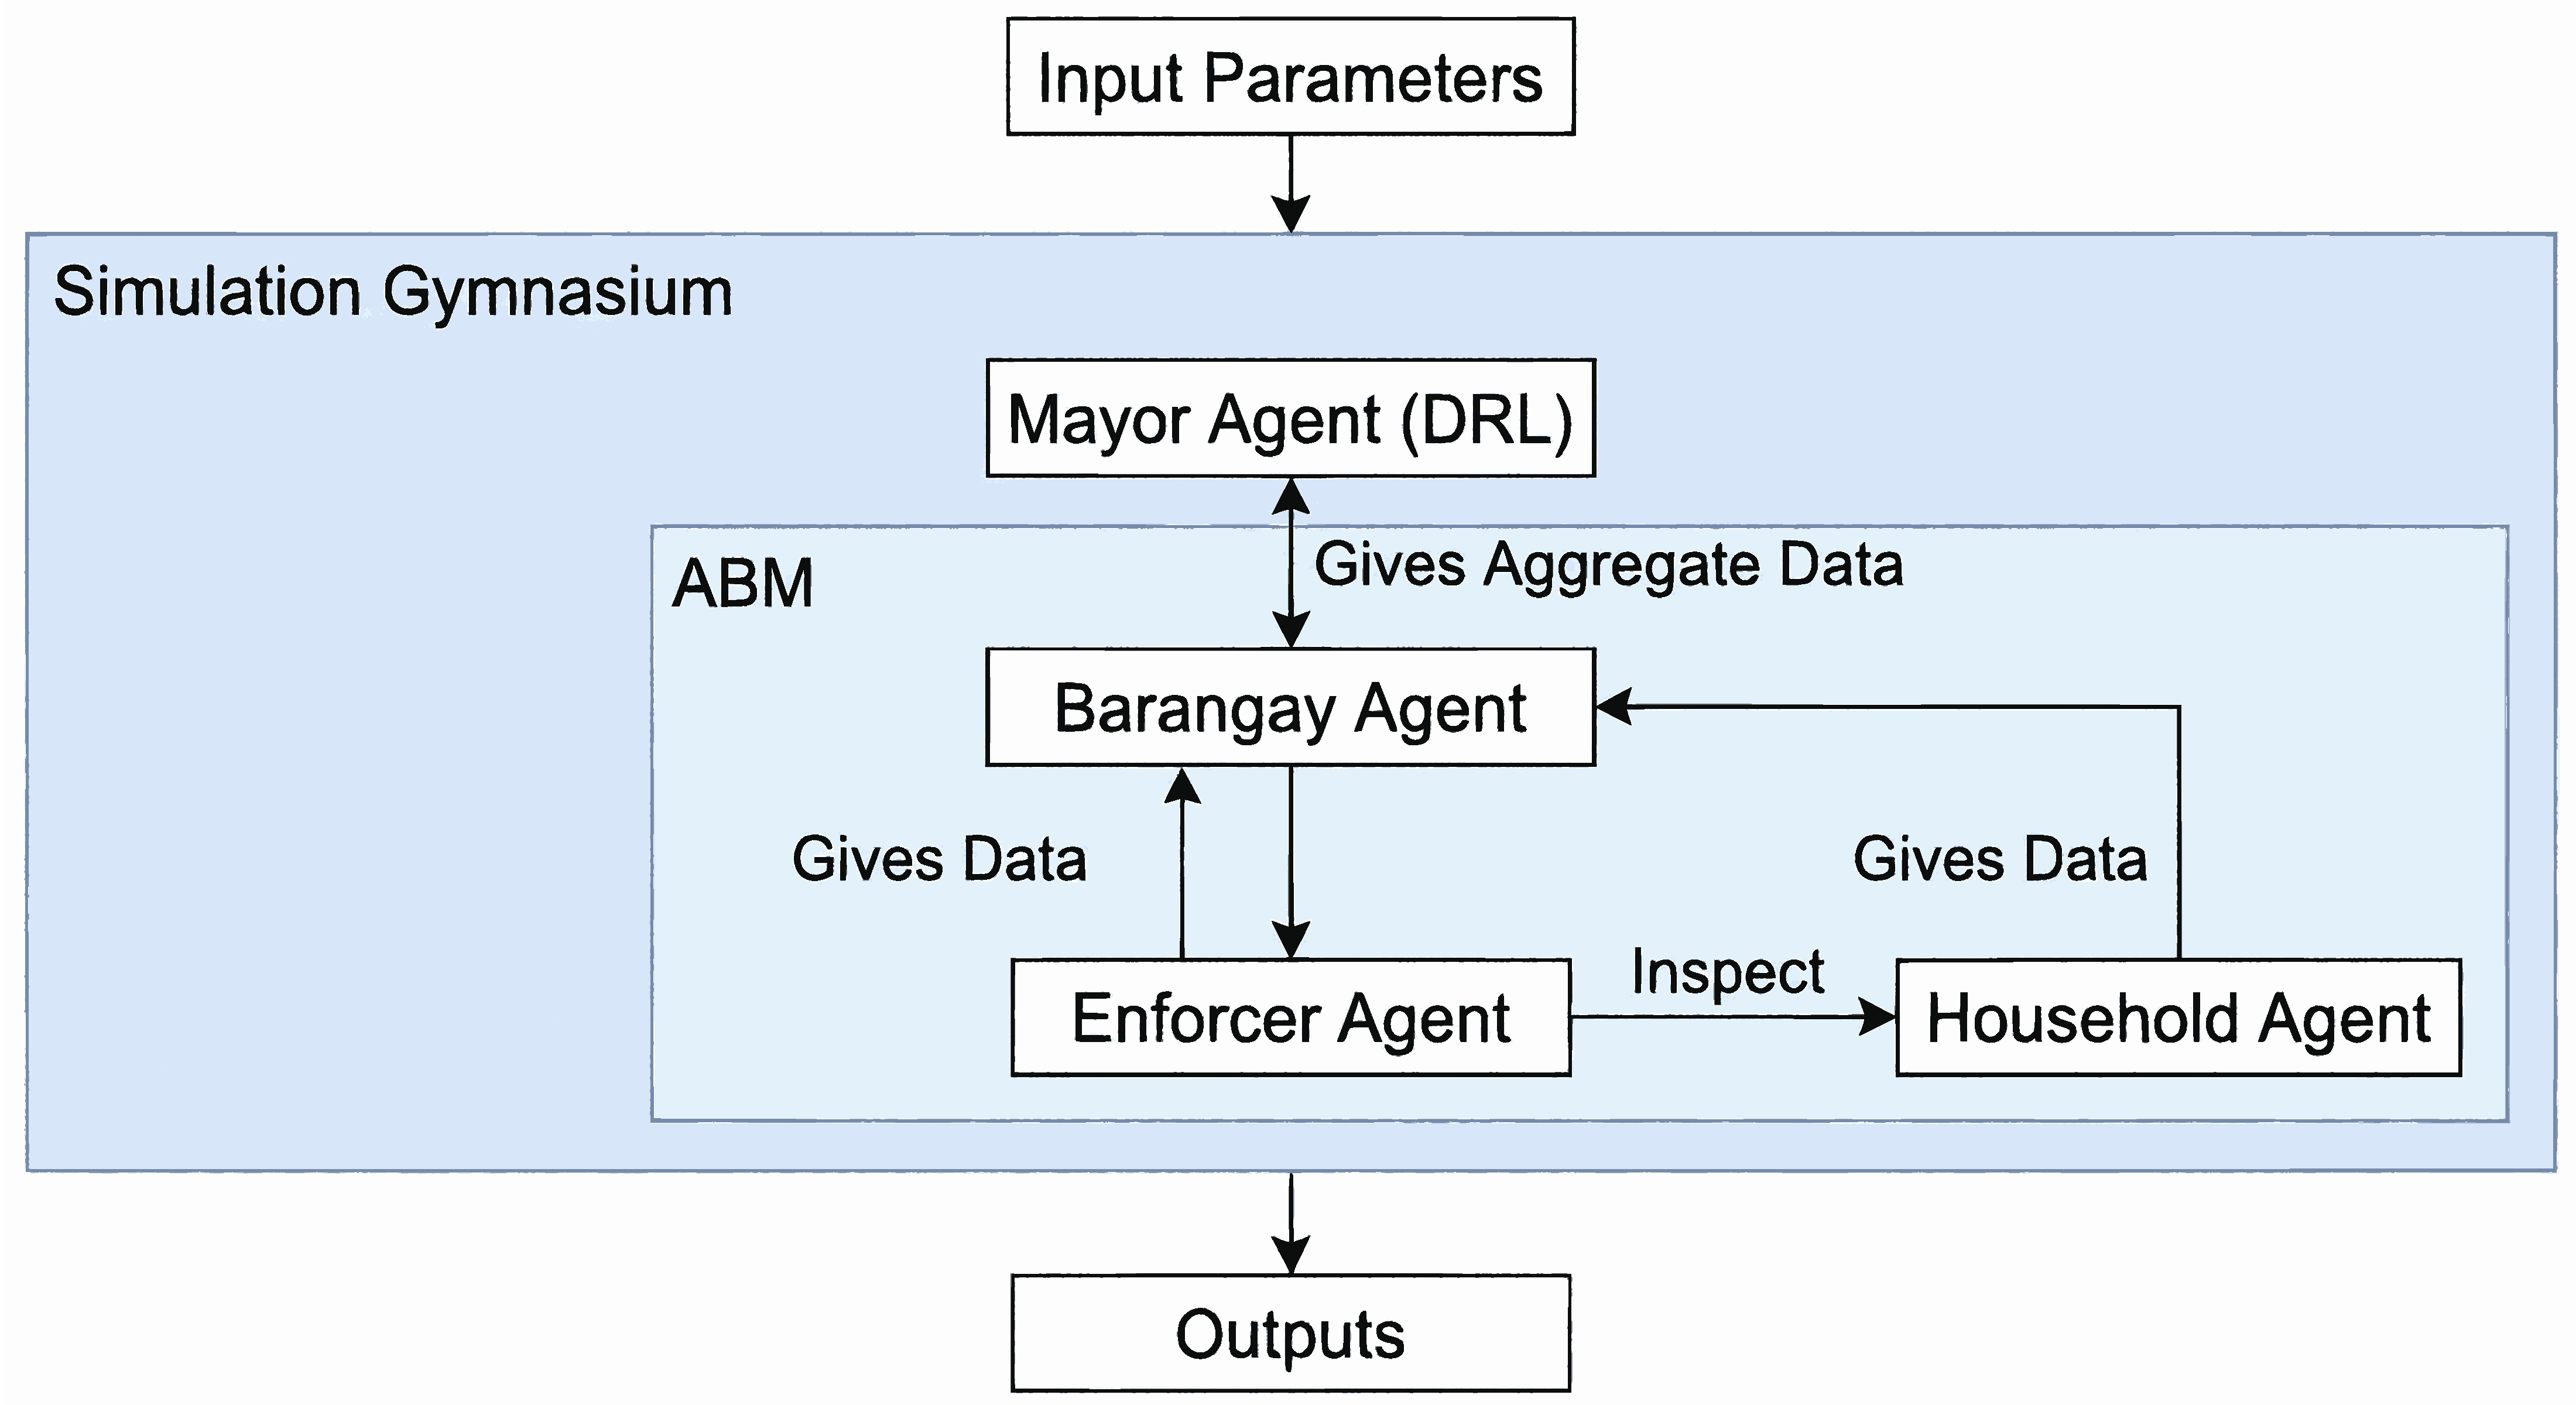
\includegraphics[width=\columnwidth]{images/simul_gym.png}
\caption{Simulation Architecture Diagram}
\label{fig:simul_diagram}
\end{figure}

\subsection{Markov Decision Process (MDP) Formulation}
To facilitate the integration of the Deep Reinforcement Learning algorithm, the entire multi-agent ecosystem is mathematically formulated as an episodic Markov Decision Process (MDP), defined by the tuple $\langle \mathcal{S}, \mathcal{A}, \mathcal{P}, \mathcal{R}, \gamma \rangle$:
\begin{itemize}
    \item \textbf{State Space ($\mathcal{S}$):} A continuous vector representing the aggregated quarterly compliance rate of each barangay, the remaining LGU budget, and the current simulation time step.
    \item \textbf{Action Space ($\mathcal{A}$):} The continuous allocation percentages of the quarterly budget across three levers (Enforcement, Incentives, Education) mapped to specific barangays.
    \item \textbf{Transition Dynamics ($\mathcal{P}$):} The non-deterministic socio-behavioral evolution of the ABM environment in response to $\mathcal{A}$.
\end{itemize}

\subsection{Multi-Level ABM Architecture}

\subsubsection{Household Agents}
Household agents are the core decision-making entities, executing binary waste segregation choices. Their cognition is governed by a dynamically weighted Theory of Planned Behavior (TPB) utility equation ($U_{seg}$):
\begin{equation}
U_{seg} = (w_{A}(t)A) + (w_{SN}(t)SN_{loc}) + (w_{PBC}(t)PBC) - C_{Net} + \epsilon
\end{equation}
Where $A$, $SN_{loc}$, and $PBC$ represent Attitude, localized Subjective Norms, and Perceived Behavioral Control. The Net Cost ($C_{Net}$) characterizes the physical and financial friction of compliance, factoring in household income sensitivity ($\gamma$), LGU incentives ($I$), and potential fines ($F$). 

To accurately model behavioral inertia, we instituted a 70\% Norm Internalization threshold. Once a community's localized compliance ($SN_{loc}$) exceeds 0.70, a damping factor mathematically restricts the decay rate of the agents' pro-environmental attitude, successfully simulating real-world ``Cultural Inertia.''

\subsubsection{Enforcement Agents (Operational Arm)}
The enforcement architecture distinguishes between Macro Enforcers (LGU-level dispatchers) and Base Enforcers (field personnel). Utilizing spatial computing, Base Enforcers execute stochastic inspections within bounded operational radii. Due to bounded rationality, they cannot inspect every household, creating a probabilistic detection rate ($P_{Detect}$) that directly alters the Household Agent's perceived risk in the $C_{Net}$ equation.

\subsubsection{Barangay Agents}
Representing the demographic zones, these agents act as localized administrative nodes. They aggregate household behavior data into compliance metrics and pass the compiled state representation up to the centralized MDP layer for evaluation.

\subsection{Mayor Agent with Heuristic-Guided DRL (HuDRL)}

\subsubsection{Proximal Policy Optimization}
The LGU policymaker (the ``Mayor Agent'') is powered by an Actor-Critic Proximal Policy Optimization (PPO) neural network. The Actor network outputs continuous budget allocations bounded by a Softmax normalization layer to ensure the P1,500,000 fiscal limit is never breached.

\subsubsection{Multi-Objective Reward Shaping}
Directing human behavior introduces the ``Sparse Reward Problem,'' where delayed causal effects cause standard AI agents to fail. To overcome this, the MDP utilizes a composite reward function ($R_{total}$):
\begin{equation}
R_{total} = w_{1}R_{Comp} + w_{2}R_{Sustain} - w_{3}P_{Backlash} + R_{Shaping}
\end{equation}
This balances environmental compliance ($R_{Comp}$) against fiscal sustainability ($R_{Sustain}$) and public pushback ($P_{Backlash}$). 

\subsubsection{Targeted Amplification Algorithm}
To prevent the PPO agent from falling into the sub-optimal trap of equitable distribution, $R_{Shaping}$ provides a massive heuristic bonus for concentrating $>40\%$ of the budget on a single failing node. This logic is executed via Algorithm 1.

\begin{algorithm}[H]
\caption{HuDRL Targeted Amplification}\label{alg:hudrl}
\begin{algorithmic}[1]
\STATE \textbf{Input:} State $S_t$, Quarterly Budget $B_{cap}$
\STATE $B_{crit} \leftarrow \arg\min_{b} (\text{compliance\_rate})$
\STATE $A_{raw} \leftarrow \pi_{\theta}(S_t)$ \COMMENT{Actor NN Policy}
\IF{$A_{raw}[B_{crit}] > \delta_{intent}$}
    \STATE $A_{raw}[B_{crit}] \leftarrow A_{raw}[B_{crit}] \times 100$ \COMMENT{Amplify Focus}
\ENDIF
\STATE $A_{final} \leftarrow \text{Softmax}(A_{raw}) \times B_{cap}$
\STATE Execute $A_{final}$ within ABM Environment
\STATE $R_{total} \leftarrow R_{base} + R_{Shaping\_Bonus}$
\STATE Update PPO Actor-Critic Networks
\end{algorithmic}
\end{algorithm}

\section{Results and Discussion}

\subsection{Data Gathered and Calibration}
Empirical calibration successfully reconciled an ``Act vs. Reality'' discrepancy. While interviews with local officials suggested perceived compliance rates of 40-50\%, MENRO audits confirmed actual compliance was 10-15\%. The model utilized Barangay Poblacion (at an audited 2\% compliance) as a high-fidelity anchor to counteract social desirability bias, establishing a valid Status Quo baseline.

\begin{table}[htbp]
\caption{Synthesized Barangay Profiles and Baselines}
\begin{center}
\begin{tabular}{lcccc}
\toprule
\textbf{Barangay} & \textbf{Pop.} & \textbf{Quarterly Cap} & \textbf{Initial Comp.} & \textbf{$C_{Effort}$} \\
\midrule
Poblacion & 1,534 & P50,000 & 2\% & 0.20 \\
Liangan East & 608 & P7,500 & 14\% & 0.60 \\
Ezperanza & 574 & P22,500 & 14\% & 0.70 \\
Binuni & 507 & P31,592 & 15\% & 0.80 \\
Demologan & 463 & P5,250 & 11\% & 0.60 \\
Babalaya & 171 & P3,750 & 14\% & 0.90 \\
Mati & 165 & P20,000 & 11\% & 0.50 \\
\bottomrule
\end{tabular}
\label{tab:profiles}
\end{center}
\end{table}

\subsection{Global Sensitivity Analysis on Household Agents}
A Sobol Global Sensitivity Analysis (GSA) revealed that the ``Cost of Effort'' ($C_{effort}$) is the overwhelmingly dominant driver of behavior, accounting for 78\% of the variance in global compliance ($S_1 \approx 0.78$). This mathematically validates the ``Convenience Hypothesis''—if the physical or financial friction of segregation is high, households will default to non-compliance regardless of environmental beliefs. Conversely, the intrinsic Attitude weight ($w_a$) exhibited near-zero sensitivity. This quantifies the ``Value-Action Gap,'' proving that Information and Education Campaigns (IEC) have a strictly limited ceiling of effectiveness when deployed without localized structural support.

\begin{figure}[htbp]
\centering
% Changed \textwidth to \columnwidth to fit properly inside the IEEE double-column layout
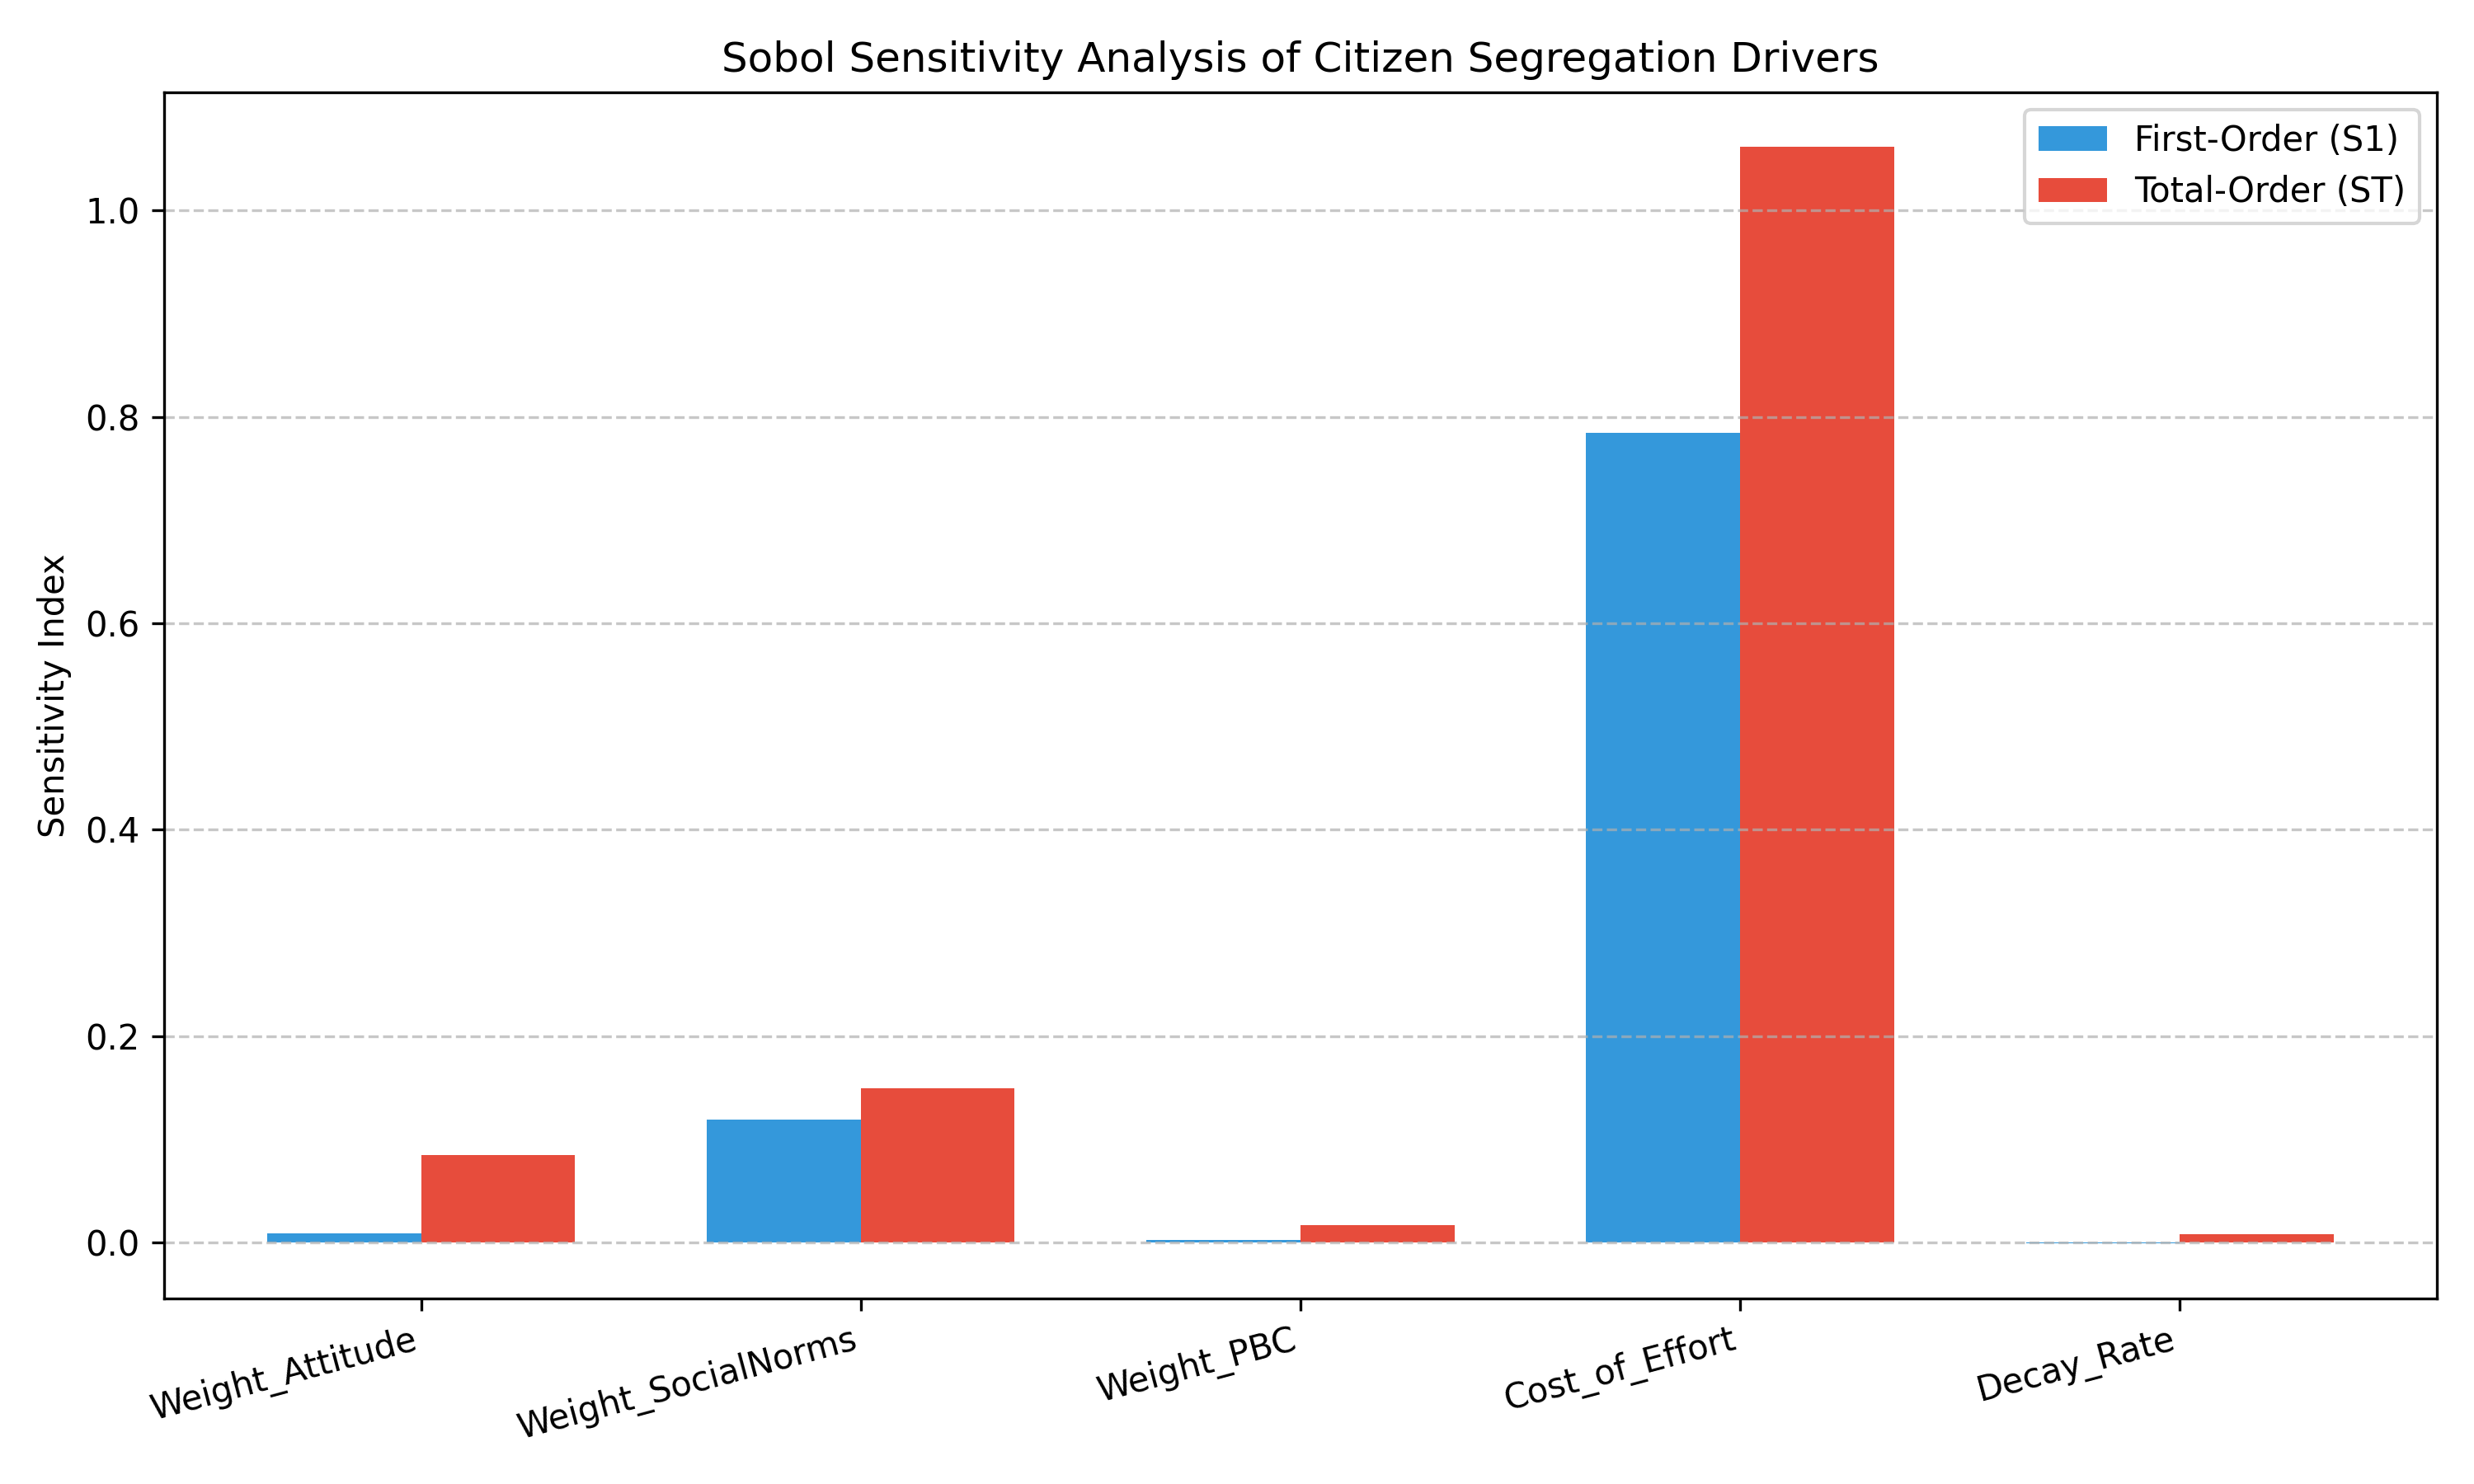
\includegraphics[width=\columnwidth]{images/Sobol.png}
\caption{General Sensitivity Analysis using the Sobol Method}
\label{fig:sobol}
\end{figure}

\subsection{Comparative Analysis of Policy Strategies}
Simulation experiments over a three-year horizon demonstrated a stark divergence between traditional heuristics and DRL optimization. The ``Status Quo'' baseline policy, which distributed the municipal budget equally across the barangays, acted as a dilution mechanism. Funds were spread too thin to cross the behavioral tipping point, resulting in a terminal global compliance of only 57.1\%.

\begin{figure}[htbp]
\centering
% Changed \textwidth to \columnwidth to fit properly inside the IEEE double-column layout
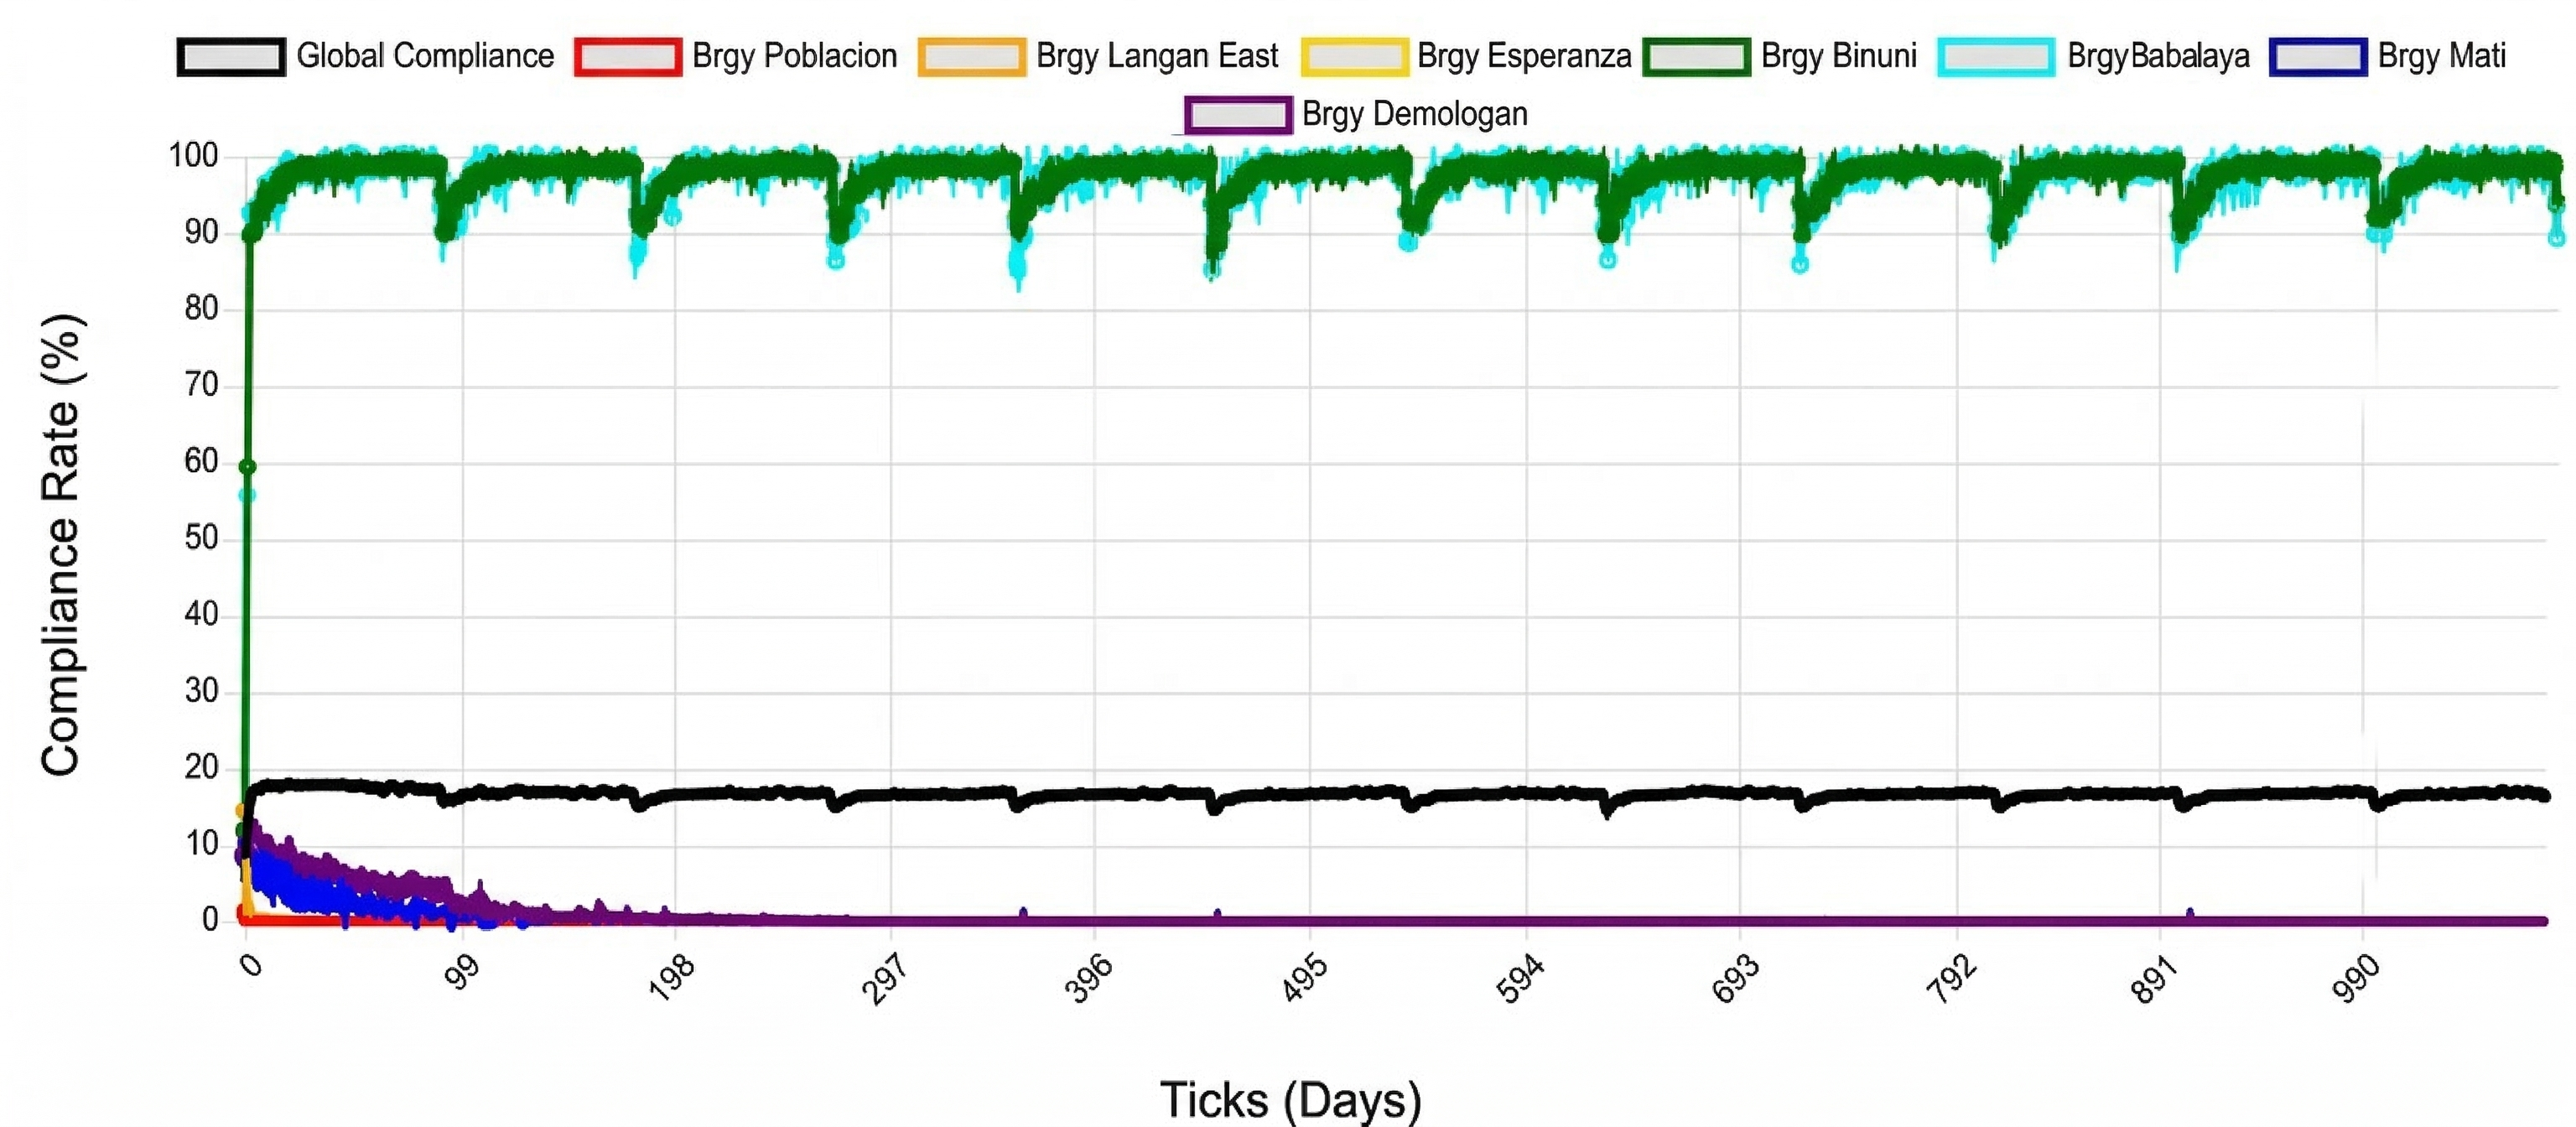
\includegraphics[width=\columnwidth]{images/Baseline.png}
\caption{Compliance Rate of Baseline Performance under Pure IEC Strategy}
\label{fig:baseline_graph}
\end{figure}

In contrast, the HuDRL Mayor Agent autonomously discovered an aggressive ``Sequential Saturation'' strategy, achieving 92.8\% global compliance. By bypassing human intuitive biases toward ``fair'' simultaneous distribution, the AI concentrated up to 69\% of its budget onto single barangays sequentially. After pushing a locale past the 70\% norm internalization threshold, the AI effectively triggered the Graduation Effect. It then ceased funding that stabilized area—relying entirely on cultural inertia to prevent behavioral decay—and pivoted its fiscal arsenal to besiege the next municipal bottleneck.

\begin{figure}[htbp]
\centering
% Changed \textwidth to \columnwidth to fit properly inside the IEEE double-column layout
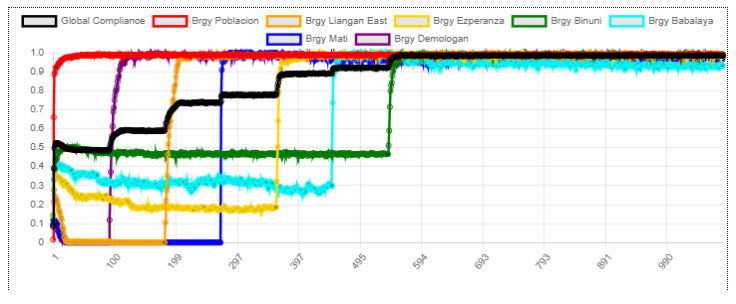
\includegraphics[width=\columnwidth]{images/ppo_result.png}
\caption{Compliance Rate of Heuristic-Guided Deep Reinforcement Learning Strategy}
\label{fig:hudrl_graph}
\end{figure}

\section{Conclusion}
This study proves that coupling Agent-Based Modeling with Heuristic-Guided DRL provides a powerful, risk-free virtual laboratory for optimizing complex public policy. By formulating the Municipality of Bacolod as an MDP, the AI demonstrated that overcoming logistical friction through targeted, sequential saturation of resources is mathematically superior to broad, diluted educational mandates. Future work will explore expanding this architecture into Multi-Agent Reinforcement Learning (MARL), allowing barangays to operate as autonomous sub-agents dynamically negotiating for LGU funding.

\section*{Acknowledgment}
The authors extend their deepest gratitude to the Bacolod LGU for providing essential audit data. Furthermore, we express our sincere thanks to Department of Computer Science, College of Computer Studies of MSU-IIT, for the support and guidance.

\begin{thebibliography}{00}

\bibitem{ra9003} Republic of the Philippines, ``Ecological Solid Waste Management Act of 2000, Rep. Act No. 9003,'' Jan. 2001.

\bibitem{tian2024} X. Tian, et al., ``Agent-based modeling in solid waste management: Advantages, progress, challenges and prospects,'' \textit{Env. Impact Assess. Rev.}, vol. 110, p. 107723, 2024.

\bibitem{centola2018} D. Centola, J. Becker, D. Brackbill, and A. Baronchelli, ``Experimental evidence for tipping points in social convention,'' \textit{Science}, vol. 360, no. 6393, pp. 1116--1119, 2018.

\bibitem{andre2021} P. Andre, T. Boneva, F. Chopra, and A. Falk, ``Fighting climate change: The role of norms, preferences, and moral values,'' \textit{Working Paper}, 2021.

\bibitem{paigalan2025} S. J. L. Paigalan, et al., ``Knowledge, attitude, and practices on solid waste management among residents of a riverside barangay,'' \textit{Scientia}, vol. 2, no. 5, pp. 3--14, 2025.

\bibitem{zhao2022} A. Zhao, L. Zhang, X. Ma, F. Gao, and H. Zhu, ``Effectiveness of extrinsic incentives for promoting rural waste sorting in developing countries,'' \textit{The Developing Economies}, vol. 60, no. 3, 2022.

\bibitem{taraghi2025} M. Taraghi and L. Yoder, ``Integrating the theory of planned behavior in agent-based models: A systematic review,'' \textit{Ecological Modelling}, vol. 508, p. 111231, 2025.

\bibitem{zheng2022b} S. Zheng, et al., ``The AI Economist: Taxation policy design via two-level deep multiagent reinforcement learning,'' \textit{Science Advances}, vol. 8, no. 18, 2022.

\end{thebibliography}

\end{document}